\documentclass[11pt, oneside, numbers=noenddot]{scrbook}
\usepackage{amstex}
\usepackage{geometry}
%\usepackage{german}
%\usepackage{ngerman}
\usepackage[english]{babel}
\usepackage[parfill]{parskip}                % Activate to begin paragraphs with an empty line rather than an indent
\usepackage{graphicx}                        % Use pdf, png, jpg, or epsß with pdflatex; use eps in DVI mode
% TeX will automatically convert eps --> pdf in pdflatex

%\usepackage{helvet}						% Kommentar wegnehmen, um in Helvetica zu schreiben
%\renewcommand{\familydefault}{\sfdefault}
%\fontfamily{phv}\selectfont

\usepackage[version=4]{mhchem}
\usepackage{chemfig}

\usepackage{amssymb}
\usepackage{mathtools} % includes amsmath

\usepackage[utf8]{inputenc}
\usepackage[T1]{fontenc}

\usepackage{lscape}

%\usepackage{arydshln} attention: not compatible with longtable
\usepackage{tabularx}
\usepackage{longtable} % table over multiple pages
\usepackage{multirow}
\usepackage{subfig}
\usepackage{pdfpages}
\usepackage{framed}

\usepackage{forloop}
\usepackage{listings}
\usepackage{fancyvrb}
\usepackage{color}
\usepackage{colortbl}
\usepackage{courier}
\usepackage{pifont}

\usepackage[pdftex]{hyperref}
\usepackage{url}

\usepackage{float} % für \begin{figure}[H]
\usepackage{fancyhdr}
\usepackage{lipsum}

\usepackage{multicol} % für mehrspaltige Texte


%	%%%%%%%%%%%%%%%%%%%%%%%%%%%%%%%%%%%%%%%%%%%%%%%%%%%%%%%%
% 	Vermeiden der KOMA Script Fehlermeldung:
%      'Class scrbook Error: undefined old font command `\rm''	
%	%%%%%%%%%%%%%%%%%%%%%%%%%%%%%%%%%%%%%%%%%%%%%%%%%%%%%%%%

\makeatletter
\DeclareOldFontCommand{\rm}{\normalfont\rmfamily}{\mathrm}
\DeclareOldFontCommand{\sf}{\normalfont\sffamily}{\mathsf}
\DeclareOldFontCommand{\tt}{\normalfont\ttfamily}{\mathtt}
\DeclareOldFontCommand{\bf}{\normalfont\bfseries}{\mathbf}
\DeclareOldFontCommand{\it}{\normalfont\itshape}{\mathit}
\DeclareOldFontCommand{\sl}{\normalfont\slshape}{\@nomath\sl}
\DeclareOldFontCommand{\sc}{\normalfont\scshape}{\@nomath\sc}
\makeatother


%	%%%%%%%%%%%%%%%%%%%%%%%%%%%%%%%%%%%%%%%%%%%%%%%%%%%%%%%%
% 	Dokumentabmessungen	
%	%%%%%%%%%%%%%%%%%%%%%%%%%%%%%%%%%%%%%%%%%%%%%%%%%%%%%%%%

\geometry {a4paper, bottom=30mm, right=25mm}%, left=30mm, right=30mm, top=25mm, bottom=25mm}


%	%%%%%%%%%%%%%%%%%%%%%%%%%%%%%%%%%%%%%%%%%%%%%%%%%%%%%%%%
% 	Kopfzeile
%	%%%%%%%%%%%%%%%%%%%%%%%%%%%%%%%%%%%%%%%%%%%%%%%%%%%%%%%%

\pagestyle{fancyplain}
\fancyhf{}

% Kopfzeile links: Kapitel rechts: HTL Logo
\lhead{\fancyplain{}{\nouppercase\leftmark}}
\rhead{\fancyplain{}{
\includegraphics[width=0.9cm]{./media/images/htl_c_cmyk_rein}}}

\cfoot{\fancyplain{\thepage}{}}
\rfoot{\fancyplain{}{\thepage}}


% Auskommentieren der folgenden Zeile setzt das HTL Logo in die
% Mitte der Kopfzeile auf jeder ersten Haupt-Kapitelseite

%\chead{\fancyplain{
\includegraphics[width=1.5cm]{./media/images/htl_c_cmyk_rein.pdf}}{}}


%	%%%%%%%%%%%%%%%%%%%%%%%%%%%%%%%%%%%%%%%%%%%%%%%%%%%%%%%%
% 	Farbdefinitionen	
%	%%%%%%%%%%%%%%%%%%%%%%%%%%%%%%%%%%%%%%%%%%%%%%%%%%%%%%%%

\definecolor{grey}{RGB}{127,127,127}
\definecolor{lightgrey}{RGB}{180,180,180}
\definecolor{dkgreen}{rgb}{0,0.6,0}
\definecolor{gray}{rgb}{0.5,0.5,0.5}
\definecolor{mauve}{rgb}{0.58,0,0.82}

\definecolor{cssId}{rgb}        {0,0,0.6 }%{0.75, 0.00, 0.00 }
\definecolor{cssAttribute}{rgb}    {0.58,0,0.82 }%{0.00, 0.00, 0.75 }
\definecolor{cssClass}{rgb}        {0,0,0.6 }%{0.00, 0.75, 0.00 }
\definecolor{cssComment}{rgb}    {0,0.6,0 }%{0.00, 0.75, 0.00 }
\definecolor{cssString}{rgb}    {0.6,0,0 }%{0.00, 0.75, 0.00 }


%	%%%%%%%%%%%%%%%%%%%%%%%%%%%%%%%%%%%%%%%%%%%%%%%%%%%%%%%%
% 	Diverse Befehle		
%	%%%%%%%%%%%%%%%%%%%%%%%%%%%%%%%%%%%%%%%%%%%%%%%%%%%%%%%%

%	Quelltext im Textfluss
\def\inlinecode#1{\texttt{\color{gray}{#1}}}


%	Paragraph mit Zeilenumbruch nachher
\def\htlParagraph#1{\paragraph*{#1}$\;$ \\}

%   Short Version of \today
\newcommand{\leadingzero}[1]{\ifnum #1<10 0\the#1\else\the#1\fi}
\newcommand{\todayshort}{\leadingzero{\day}.\leadingzero{\month}.\the\year}

%	%%%%%%%%%%%%%%%%%%%%%%%%%%%%%%%%%%%%%%%%%%%%%%%%%%%%%%%%
% 	Code Formatierung		
%	%%%%%%%%%%%%%%%%%%%%%%%%%%%%%%%%%%%%%%%%%%%%%%%%%%%%%%%%
\lstset{literate=%
    {Ö}{{\"O}}1
    {Ä}{{\"A}}1
    {Ü}{{\"U}}1
    {ß}{{\ss}}2
    {ü}{{\"u}}1
    {ä}{{\"a}}1
    {ö}{{\"o}}1
}

\lstset{ % 
%  language=Octave,                			% the language of the code 
    basicstyle=\ttfamily\footnotesize,        % the size of the fonts that are used for the code
    numbers=left,                        % where to put the line-numbers
    numberstyle=\tiny\color{gray},        % the style that is used for the line-numbers
    stepnumber=1,                        % the step between two line-numbers. If it's 1, each line
% will be numbered
    numbersep=5pt,                        % how far the line-numbers are from the code
    backgroundcolor=\color{white},            % choose the background color. You must add \usepackage{color}
    showspaces=false,                    % show spaces adding particular underscores
    showstringspaces=false,                % underline spaces within strings
    showtabs=false,                        % show tabs within strings adding particular underscores
%	frame=single,                   		% adds a frame around the code
    frame=l,
    rulecolor=\color{dkgreen},                % if not set, the frame-color may be changed on line-breaks within not-black text (e.g. comments (green here))
    tabsize=2,                            % sets default tabsize to 2 spaces
    captionpos=b,                        % sets the caption-position to bottom
    breaklines=true,                        % sets automatic line breaking
    breakatwhitespace=false,                % sets if automatic breaks should only happen at whitespace
%	title=\lstname,                   		% show the filename of files included with \lstinputlisting;
% also try caption instead of title
    keywordstyle=\color{blue},            % keyword style
    commentstyle=\color{dkgreen},        % comment style
    stringstyle=\color{mauve},                % string literal style
    escapeinside={\%*}{*)},                    % if you want to add LaTeX within your code
morekeywords={*,...},                    % if you want to add more keywords to the set
deletekeywords={...}                    % if you want to delete keywords from the given language
}

%	%%%%%%%%%%%%%%%%%%%%%%%%%%%%%%%%%%%%%%%%%%%%%%%%%%%%%%%%
% 	CSS		
\lstdefinelanguage{CSS}{
alsoletter={\\,/,*,:,-,\#,.},
identifierstyle=\idstyle,
keywords={accelerator:, azimuth:, background:, background-attachment:, background-color:, background-image:, background-position:, background-position-x:, background-position-y:, background-repeat:, behavior:, border:, border-bottom:, border-bottom-color:, border-bottom-style:, border-bottom-width:, border-collapse:, border-color:, border-left:, border-left-color:, border-left-style:, border-left-width:, border-right:, border-right-color:, border-right-style:, border-right-width:, border-spacing:, border-style:, border-top:, border-top-color:, border-top-style:, border-top-width:, border-width:, bottom :, caption-side:, clear:, clip:, color:, content:, counter-increment:, counter-reset:, cue:, cue-after:, cue-before:, cursor:, direction:, display:, elevation:, empty-cells :, filter:, float:, font:, font-family:, font-size:, font-size-adjust:, font-stretch:, font-style:, font-variant:, font-weight:, height:, ime-mode:, include-source:, layer-background-color:, layer-background-image:, layout-flow:, layout-grid:, layout-grid-char:, layout-grid-char-spacing:, layout-grid-line:, layout-grid-mode:, layout-grid-type:, left:, letter-spacing:, line-break:, line-height:, list-style:, list-style-image:, list-style-position:, list-style-type:, margin:, margin-bottom:, margin-left:, margin-right:, margin-top:, marker-offset:, marks:, max-height:, max-width:, min-height:, min-width:, -moz-binding:, -moz-border-radius:, -moz-border-radius-topleft:, -moz-border-radius-topright:, -moz-border-radius-bottomright:, -moz-border-radius-bottomleft:, -moz-border-top-colors:, -moz-border-right-colors:, -moz-border-bottom-colors:, -moz-border-left-colors:, -moz-opacity:, -moz-outline:, -moz-outline-color:, -moz-outline-style:, -moz-outline-width:, -moz-user-focus:, -moz-user-input:, -moz-user-modify:, -moz-user-select:, orphans:, outline:, outline-color:, outline-style:, outline-width:, overflow:, overflow-X:, overflow-Y:, padding:, padding-bottom:, padding-left:, padding-right:, padding-top:, page:, page-break-after:, page-break-before:, page-break-inside:, pause:, pause-after:, pause-before:, pitch:, pitch-range:, play-during:, position:, quotes:, -replace:, richness:, right:, ruby-align:, ruby-overhang:, ruby-position:, -set-link-source:, size:, speak:, speak-header:, speak-numeral:, speak-punctuation:, speech-rate:, stress:, scrollbar-arrow-color:, scrollbar-base-color:, scrollbar-dark-shadow-color:, scrollbar-face-color:, scrollbar-highlight-color:, scrollbar-shadow-color:, scrollbar-3d-light-color:, scrollbar-track-color :, table-layout:, text-align:, text-align-last:, text-decoration:, text-indent:, text-justify:, text-overflow:, text-shadow:, text-transform:, text-autospace:, text-kashida-space:, text-underline-position:, top:, unicode-bidi:, -use-link-source:, vertical-align:, visibility:, voice-family:, volume :, white-space:, widows:, width:, word-break:, word-spacing:, word-wrap:, writing-mode},
keywordstyle=\color{cssAttribute},%\bfseries,
ndkeywords={@import, @media, @page, @font-face, @charset, @namespace, a, html, body, title, pre, h1, h2, h3, h4, h5, h6, ul, ol, li, p, br, blockquote, dl, dt, dd, div, img, strong, em, cite, tt, i, b, table, tr, td, th, frame, form, option, input, button, nav, section, article, aside, footer, hr, sup, sub, del, ins, small, span},
ndkeywordstyle=\color{cssId},%,\bfseries,
%        identifierstyle=\color{black},
%        sensitive=false,
%        comment=[l]{//},
morecomment=[s]{/*}{*/},
commentstyle=\color{cssComment}\ttfamily,
stringstyle=\color{cssString}\ttfamily,
morestring=[b]',
morestring=[b]"
}

\makeatletter
\newcommand*\idstyle[1]{%
\expandafter\id@style\the\lst@token{#1}\relax%
}

\def\id@style#1#2\relax{%
\ifnum\pdfstrcmp{#1}{\#}=0%
\small\ttfamily\color{cssId} \the\lst@token%
\else%
\ifnum\pdfstrcmp{#1}{.}=0%
\small\ttfamily\color{cssClass} \the\lst@token%
\else%
\ifnum\pdfstrcmp{#1}{:}=0%
\small\ttfamily\color{cssAttribute} \the\lst@token%
\else%
%\edef\tempa{\uccode#1}%
\edef\tempa{\lccode`#1}%
\edef\tempb{`#1}%
\ifnum\tempa=\tempb%
\small\ttfamily\color{mauve} \the\lst@token%
\else%
\the\lst@token%
\fi%
\fi%
\fi%
\fi%
}
\makeatother



%	%%%%%%%%%%%%%%%%%%%%%%%%%%%%%%%%%%%%%%%%%%%%%%%%%%%%%%%%
% 	JavaScript	
\lstdefinelanguage{JavaScript}{
keywords={typeof, new, true, false, catch, function, return, null, catch, switch, var, if, in, while, do, else, case, break},
alsoletter={\{,\}\\,/,*,:,-,\#,.},
%       keywordstyle=\color{blue}\bfseries,
ndkeywords={class, export, boolean, throw, implements, import, this},
%        ndkeywordstyle=\color{darkgray}\bfseries,
%        identifierstyle=\color{black},
%        sensitive=false,
comment=[l]{//},
morecomment=[s]{/*}{*/},
%        commentstyle=\color{purple}\ttfamily,
%        stringstyle=\color{red}\ttfamily,
morestring=[b]',
morestring=[b]"
}


%	%%%%%%%%%%%%%%%%%%%%%%%%%%%%%%%%%%%%%%%%%%%%%%%%%%%%%%%%
% 	TypoScript	
\lstdefinelanguage{TypoScript}{
keywords={typeof, new, true, false, catch, function, return, null, catch, switch, var, if, in, while, do, else, case, break},
alsoletter={\{,\}\\,/,*,:,-,\#,.},
%       keywordstyle=\color{blue}\bfseries,
ndkeywords={class, export, boolean, throw, implements, import, this},
%        ndkeywordstyle=\color{darkgray}\bfseries,
%        identifierstyle=\color{black},
%        sensitive=false,
comment=[l]{//},
morecomment=[s]{/*}{*/},
%        commentstyle=\color{purple}\ttfamily,
%        stringstyle=\color{red}\ttfamily,
morestring=[b]',
morestring=[b]"
}


% Initialen der Authoren
\newcommand{\authorInitialsA}{TD} % Tobias Daxecker
\newcommand{\authorInitialsB}{MS} % Mathias Standhartinger

% Die Initialen werden verwendet um anzuzeigen wer welches Kapitel
% erstellt hat.

% Die Befehle \authorA - \authorB werden in den Kapitelüberschriften angefügt
\newcommand{\authorA}{\textmd{\textsuperscript{\authorInitialsA}}}
\newcommand{\authorB}{\textmd{\textsuperscript{\authorInitialsB}}}

% Titel der Arbeit:
\newcommand{\htlArbeitsthema}{REECYPRO}

\begin{document}

    \pagenumbering{roman}

    % !TEX root = ../Vorlage_DA.tex

%	########################################################
% 							Deckblatt
%	########################################################


\titlehead{%
\begin{minipage}[c]{0.20\linewidth}

\includegraphics[width=0.8\linewidth]{media/images/htl_c_cmyk_rein}
\end{minipage}
\begin{minipage}[c]{0.5\linewidth}
\begin{center}
{\bfseries\sffamily\large Höhere  technische  Bundeslehranstalt\\
und  Bundesfachschule\\
{\normalsize im Hermann Fuchs Bundesschulzentrum} }
\end{center}
\end{minipage}
\begin{minipage}[c]{0.2\linewidth}
\hfill 
\includegraphics[width=0.8\linewidth]{media/images/htl-bildung-mit-zukunft}
\end{minipage}\\
}
\title{\vspace{4em}\htlArbeitsthema}
\subtitle{ {\Large Diplomarbeit}\\[1em]Schulautonomer Schwerpunkt\\ Bionik}



\author{\\[3.5em] 
\emph{ausgeführt im Schuljahr 2023/2024 von:} \\[1em] 
Tobias Daxecker, 5CHELS\\[1ex] 
Mathias Standhartinger, 5CHELS\\[1ex] 
\\[4em]
\emph{Betreuer:} \\[1em]
Benjamin Seeburger, MSc.
}
\date{\vspace{3\baselineskip}\today}

\begin{titlepage}	
\maketitle
\end{titlepage}

    \chapter*{Eidesstattliche Erklärung}

Ich/Wir erkläre/n an Eides statt, dass ich/wir die vorliegende Diplomarbeit selbstständig und ohne fremde Hilfe verfasst, andere als angegebene Quellen und Hilfsmittel nicht direkt benutzt und die benutzten Quellen wörtlich und inhaltlich entnommenen Stellen als solche erkenntlich gemacht habe/n.
\vspace{3cm}

\begin{tabularx}{\textwidth}{l p{1cm} l p{1cm} X}


Braunau/Inn, \todayshort & & Tobias Daxecker & & \hrulefill \\
\emph{Ort, Datum} & & \emph{Verfasser} & & \emph{Unterschrift} \vspace{2cm}\\ 

Braunau/Inn, \todayshort & & Mathias Standhartinger & & \hrulefill \\
\emph{Ort, Datum} & & \emph{Verfasser} & & \emph{Unterschrift} \vspace{2cm}\\ 

\end{tabularx}




    \chapter*{Abstract}
\addcontentsline{toc}{chapter}{Abstract}

The rare earth elements (REEs) are metals, which are used in nearly every electronic device.
The demand for new REEs is steadily rising.
Yearly, millions of tonnes of electronic waste (e-waste) are generated.
The e-waste contains valuable metals, but most of them are not recycled.

The recycling of REEs is a challenging process that currently involves the usage of a lot of energy.
But also the mining of new REEs is not eco-friendly.
It involves the usage of strong acids that harm the environment and mining workers.

In recent years, a newly discovered protein found in a specific bacteria was found to be able to tackle the challenge of REE recycling.
The protein can take up the REEs from e-waste, like washing detergents wash dirt out of clothing.

Without any additional preparation of the e-waste other than dust the e-waste, the bacteria is capable of gathering more than 70\% of REEs out of the waste.

This could be used in the near future to recycle REEs in an eco-friendly, climate-friendly and energy-saving way.

\chapter*{Introduction}
\addcontentsline{toc}{chapter}{Introduction}

In 2021, around five million tonnes of electronic waste were generated in the EU alone, but less than 40 percent were recycled.
This waste often contains valuable metals, but currently most of them are disposed.
Some of these disposed metals are the so-called rare earth elements.
The rare earths are critical for every electronic device but they are only used in small quantities, so that conventional recycling is not a economically feasible possibility.

For every new smartphone, for example, new rare earths must be mined.
This happens mostly in countries where compliance with human and environmental rights are questionable.
The following refining of the rare earths is a very energy-consuming, environmentally harmful and climate damaging process.
For a single tonne of neodymium, the most used rare earth element, some 75 tonnes of \ce{CO2} are emitted.
But the problems do not stop there.
There are only a few places on earth were rare earths are mined, because it is mostly not economically viable because of China, who dominates the market.

The largest mine for rare earths is located in China and additionally, China is the largest producer of refined rare earths, which is then used elsewhere to produce electronics.
This means that the world's current supply of rare earth elements is largely monopolized by a country, which does not adhere to human and environmental rights.

A solution could be the recycling of rare earths from electronic waste.
However, currently established methods are either very expensive, damaging to the environment or use a lot of energy.

A promising alternative could be the usage of bacteria to recover the rare earths.
Bacteria have the advantages that they do not need a lot of energy to grow and they only need inexpensive resources to be able to grow.

In this thesis, we tested if, and how rare earth elements can be recycled from electronic waste using bacteria.
We outline how this process works and we report our findings from the actual realisation of this process.


    \tableofcontents
    \pagenumbering{arabic}

    \chapter{Introduction}

Rare Earth Elements (REEs) play a critical role in modern-day life.
They are used in nearly every device that uses electrical power to operate.
A few examples where REEs are essential are: lasers, computer monitors, electric motors, electric generators, high-power magnets, liquid crystal displays (LCDs), solar panels and many more~\cite{usageofrees}.

\begin{figure}[H]
    \centering
    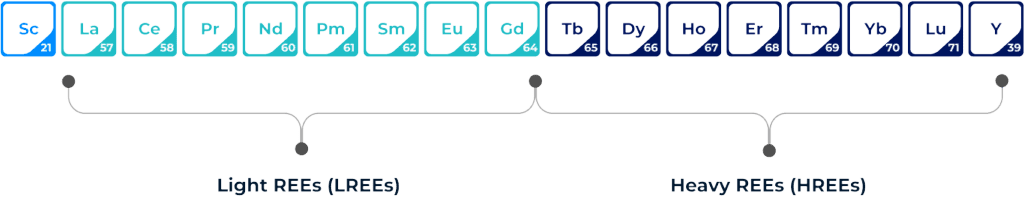
\includegraphics[width=1\textwidth]{./media/images/rees_periodic_table}
    \caption{List of all rare earth elements. Those 17 elements can be further categorized into the light rare earth elements (LREEs) and the heavy rare earth elements (HREEs). Picture from Rare Earth Industry Association / Argus Media.}
    \label{fig:list_rees}
\end{figure}


\section{Problem Setting\authorA{}}

REEs are the minerals of the future.
Almost every electronic device depends on them, but they are also crucial for the green energy transition.
For example, for every megawatthour of new wind energy generation capacity, 600 kilograms of neodymium magnets are needed~\cite{recyclingcurrent}.

Given the importance of REEs in the modern world, it is evident that the demand for them is increasing quickly.
In the coming years, as the use of electronic devices increases, many of them will become electronic waste.
It is vital for the world's future supply of rare earth elements to recycle them from this waste.


\begin{figure}[H]
    \centering
    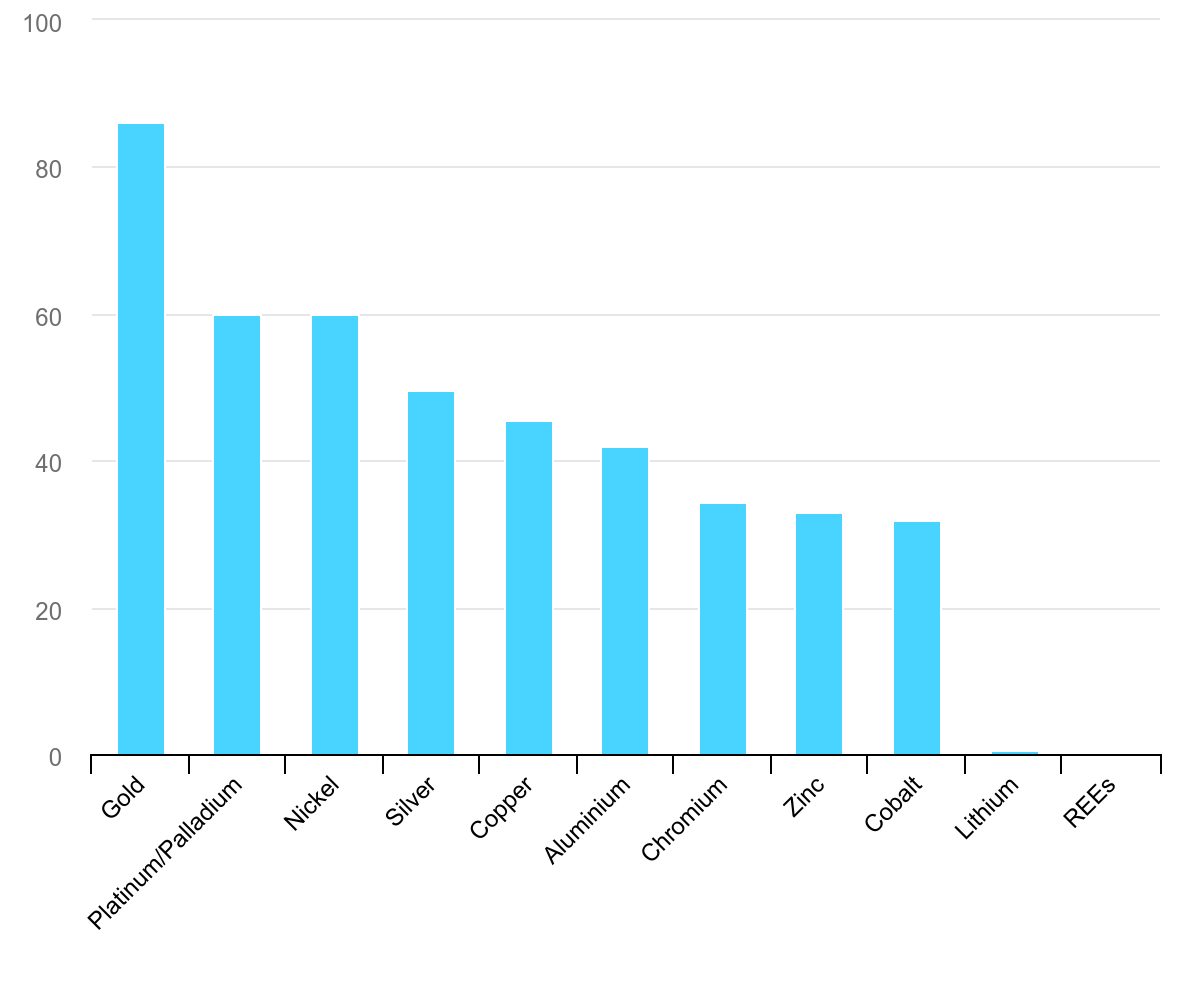
\includegraphics[width=1\textwidth]{./media/images/end-of-life-recycling-rates-for-selected-metals}
    \caption{End-of-life recycling rates of selected metals. Only 0.2\% of all produced rare earth elements are recycled. Chart from International Energy Agency~\cite{reeclimate}.}
    \label{fig:recycling_rates}
\end{figure}

Currently used recycling methods for REEs are mostly damaging to the environment and very costly~\cite{recyclingcurrent}.
Therefore, only around one percent of the global REEs supply is from recycled sources~\cite{currentrecyclingnumbers}.
The rest comes from mining, which brings its own challenges.
Rare earth ores (REOs) often contain radioactive elements which adds more complexity to the processing of the ores.
Also, the extraction of REEs is done by using a process called flotation which produces large amounts of waste water.
This waste water is highly problematic, as it often contains radioactive minerals, acids and toxic agents~\cite{reeenvimpact}.

The processing of REOs does not only damage the environment, but it also contributes to climate change.
As an example, 75 tonnes of \ce{CO2}— equivalents are emitted for every tonne of newly refined neodymium~\cite{reeclimate}.

There are already thousands of tonnes of electronic waste that contain significant amounts of REEs. Recycling them would reduce the need of mining new REOs and therefore reduce the environmental impact of new electronic devices.
Sadly, there is no easy and environmentally friendly process to recycle REEs on an industrial scale.


\section{Contributions\authorB{}}
To combat the issues mentioned above, we worked on a way to recycle REEs without the
need for large amounts of energy or resources.
By using bacteria that produce a special amino acid that allows us to bind the REEs in electronic waste, we achieved just that.
Due to the bacteria not needing significant amounts of energy, we managed to remain eco-friendly and cost-efficient.
The recycling process works by washing shredded electronic waste with our bacteria solution.
After changing the pH value of said solution we can get
the REEs back in their pure forms.
This process works on a scientific level in a laboratory but could also be used on an industrial scale using large bioreactors and washing tanks.


\section{Structure of this Thesis\authorB{}}
This thesis is divided into eight main parts, systematically addressing various aspects of
the research project. It begins with an introduction outlining the project's aims and
importance. The theoretical background section elucidates the methods and principles
underpinning the research. Practical guidance for executing the project is provided in the
experimental section. The Results and Discussion segment analyzes the project's
outcomes and implications. Project Management reflects on the planning process and
evaluates its effectiveness, accompanied by a detailed timesheet. Future Work and
Related Work suggest avenues for future research and contextualize the project within
existing literature. The conclusion summarizes key findings, challenges, and lessons
learned. Additional chapters, such as Acknowledgements, List of Figures, Bibliography,
and CV, provide further context and resources. Each section contributes to advancing
knowledge in the field, fostering scholarly discourse.


    \chapter{Theoretical Background}
In order to understand the process of the recovery of rare earth elements from electronic waste with bioaccumulation, the key procedures and techniques are described in this chapter.


\section{System Overview}
In the following section, all used methods and the most important concepts are briefly summarized.


\subsection{Detection and Measurement of REE concentration\authorA}

\subsubsection{Precipation Reactions}
A relatively simple proof if a probe contains REEs is a precipitation reaction.
The precipitation reactions a work because the rare earths form greater complexes with other molecules which have a different color than the surrounding solution ~\cite{janderblasius}.
As an example, a Ce precipitation reaction is shown in figure~\ref{fig:cer_precipitation_cropped} with an orange-red precipitate.

\begin{figure}[H]
    \centering
    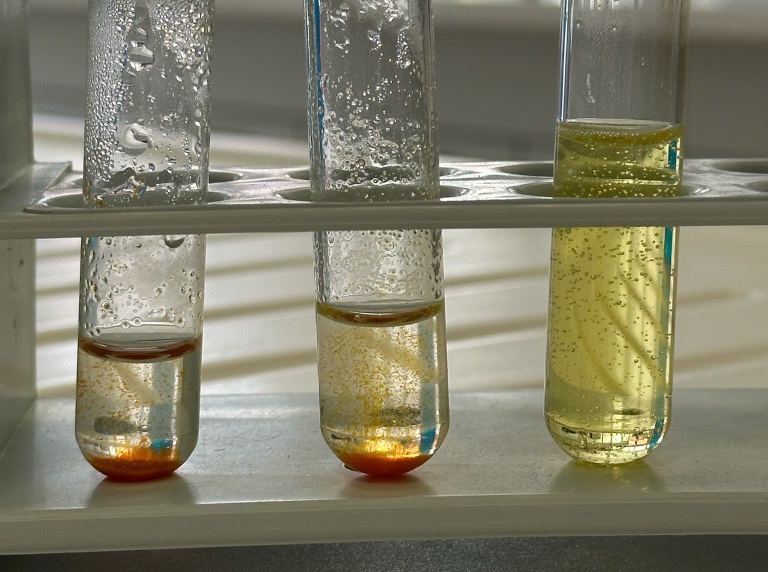
\includegraphics[width=0.8\textwidth]{./media/images/ree_precipitation_reaction_cropped}
    \caption{Precipitation of a successful REE detection reaction. The red arrows point to the orange-red precipitation.}
    \label{fig:cer_precipitation_cropped}
\end{figure}

However, you must be careful because of the REEs chemical similarity, the detection of a specific REE is not always possible with these precipitation methods.
A precipitation reaction might also not be sensitive enough for your use case.
So it could be possible that your probe contains rare earths, but you were not able to detect them.

\subsubsection{Arsenazo III Assay}
A better and more versatile method to detect rare earths in a probe is the so-called arsenazo III assay.
With this assay, it is not only possible to detect if rare earths are present, but it is also possible to determine the concentration of REEs~\cite{arsenazo3assay}.

\begin{figure}[H]
    \centering
    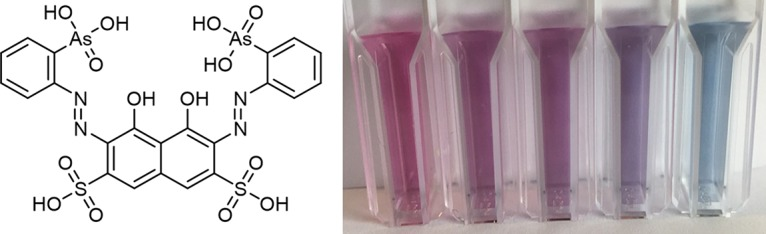
\includegraphics[width=0.9\textwidth]{media/images/arsenazo3_structure_example}
    \caption{Structure of arsenazo III. The color change of the dye depending on the REE concentration is shown on the righthandside. Picture from "Facile Arsenazo III-based assay for monitoring rare earth element depletion from cultivation media for methanotrophic and methylotrophic bacteria" Hoogendorn et al. \cite{arsenazo3assay}.}
    \label{fig:arsenazo3}
\end{figure}

Arsenazo III is a metallochromic dye.
This means that the dye changes its color depending on the presence of metal ions (for example:~\ref{fig:arsenazo3}).
A second crucial characteristic is that the color of an arsenazo III solution is also dependent on the concentration of some metal ions.
The metal ions and the arsenazo III molecule form complexes which block some certain frequencies of light.
This property can be used to determine the concentration of rare earths in a probe.

\newpage

\subsection{Methylorubrum extorquens}

\subsubsection{General information\authorB{}}

Utilizing a special strain of bacteria called \emph{Methylorubrum extorquens}, we can extract these REEs from electronic waste.
This works because the aforementioned bacteria produce an amino acid called lanmodulin which has the unique property of binding to REEs~\cite{lanmdiscovery}.
This technique allows us to wash REEs out of electronic waste in a similar way that
surfactants wash the dirt out of laundry.

\begin{figure}[H]
    \centering
    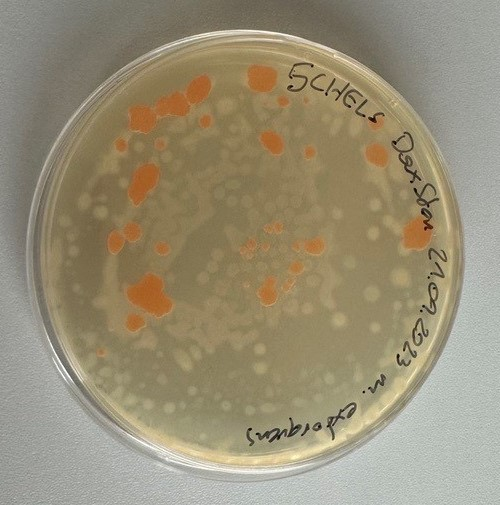
\includegraphics[width=0.8\textwidth]{./media/images/mextorquens_petri_dish}
    \caption{\emph{Methylorubrum extorquens} in a petri dish.}
    \label{fig:mextorquens_petri_dish}
\end{figure}

These bacteria reside in common soil, plant leaves, and dust and can also form symbiotic
relationships with some plants.
The bacteria appear orange or pink when cultivated on a solid or in a liquid medium.
\emph{Methylorubrum extorquens} utilizes methanol as an energy
and carbon source, which is why we had to put methanol in our nutrient media.

\subsubsection{Lanmodulin\authorA}

Lanmodulin (LanM) is a protein produced by \textit{M. extorquens}, a lanthanide-utilizing bacteria~\cite{lanmdiscovery}.
LanM is not essential for the growth or survival of \textit{M. extorquens}, and it is only produced when the bacteria are in a medium with presence of \ce{Ln^{III}} or \ce{Ce^{III}} ions~\cite{lanmroleinbiology}.
However, the mechanisms that include LanM are not understood as a whole to this day.

\begin{figure}[H]
    \centering
    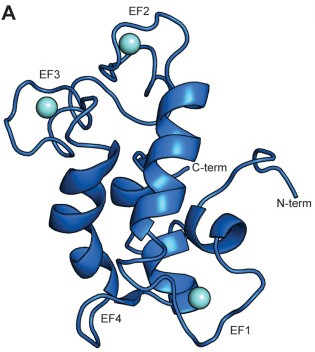
\includegraphics[width=0.6\textwidth]{./media/images/lanm_structure}
    \caption{Graphical visualization of Lanmodulins structure. EF indicates the EF-hands, this is where the REEs can bind to the protein. In this visualization, the turquoise-colored spheres are \ce{Y^{III}} ions which are bound to the EF-hands. Picture from "The biochemistry of lanthanide acquisition, trafficking and utilization", Emily R. Featherston and Joseph A. Cotruvo \cite{lanmroleinbiology}.}
    \label{fig:lanm_structure}
\end{figure}

The most important characteristic of LanM is that the molecule is able to bind lanthanide ions, primarily light REEs (LREEs).
When LanM does this, it undergoes a transformation from a disordered state to a compact form of itself.
The REEs are hereby bound to the so-called EF-hands which favor to bind to \ce{Ln^{III}} and other lanthanoids over \ce{Ca^{II}} which is usually associated with these EF-hands~\cite{lanmstructure}.


\subsubsection{Cell Lysis\authorB{}}


\subsubsection{Protein Extraction\authorB{}}


\subsubsection{IR-Spectrometry\authorB}

\subsubsection{SDS-PAGE\authorB{}}

    \section{Detection and Measurement of REE concentration\authorA{}}

%Rare Earth Elements (for short: REEs) play a critical role in modern-day life.
%They are used in nearly every device that uses electrical power to operate.
%A few example where REEs are essential are: lasers, computer monitors, electric motors, high-power magnets, liquid crystal displays (LCDs), solar panels~\cite{usageofrees}.
%In this context, it is clear that the demand for REEs is rising rapidly.
%In the following years, with more and more electronic devices produced, most of them will eventually end as electronic waste.
%Recycling REEs from this waste is crucial for the worlds REE supply.
%Current recycling methods are mostly harmful to the environment and very costly~\cite{recyclingcurrent}.
%But new recycling methods have emerged in the last years and one of them, using the technique of biosorption, is the subject of this thesis.
%To understand how this process works, it is important to know the following techniques.

The detection of rare earth elements in a sample is a crucial step in our work.
It allows us to quantify the effectiveness of our process.

In modern chemistry,
qualitative and quantitative analysis of elements in a sample is usually done with inductively coupled plasma mass spectroscopy (ICP-MS) or atom absorption spectroscopy (AAS).
However, as the ICP-MS and AAS use machines that are very, very expensive,
these methods were not an option as they exceeded our limited financial resources by far.
Instead, we had to search for other methods to detect and quantify rare earths.

In our work, we used two precipitation reactions and one method to quantify the concentration of REEs.


\subsection{Precipation Reactions}

\subsubsection{Cer Precipitation Reaction}
The precipitation reaction for cer works by utilizing the oxidation states +III and +IV~\cite{cerdetection,janderblasius}.

\begin{figure}[H]
    \centering
    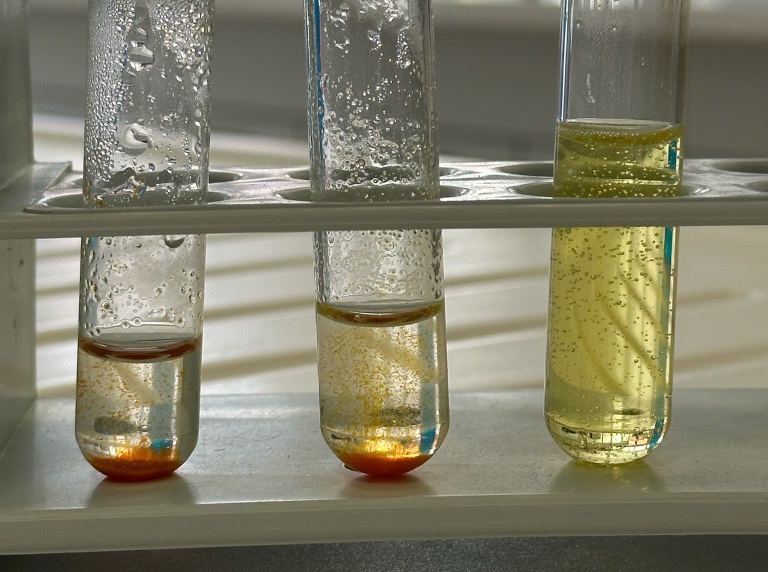
\includegraphics[width=0.9\textwidth]{./media/images/ree_precipitation_reaction_cropped}
    \caption{Precipitation of a successful cer detection reaction. The test tube on the righthandside does not show any precipitation because the sample was deionized water.}
    \label{fig:cer_precipitation_cropped1}
\end{figure}

Cer in the aforementioned states forms complexes together with \ce{H2O2}.
The complexes are called cer peroxide hydrates.
Their chemical formulas are \ce{Ce(OH)2(OOH)} and \ce{Ce(OH)3(OOH)}.
These complexes fall out of the solution as a red-brown colored precipitate.

\subsubsection{Neodymium Precipitation Reaction}
The reaction to detect neodymium is a bit more complicated.
It also uses the +III oxidation state of neodymium.
The neodymium reacts with acetic acid to form neodymium acetate.
As the last step, iodide is given to the solution which forms a blue-colored complex together with the neodymium acetate~\cite{janderblasius}.

\begin{figure}[H]
    \centering
    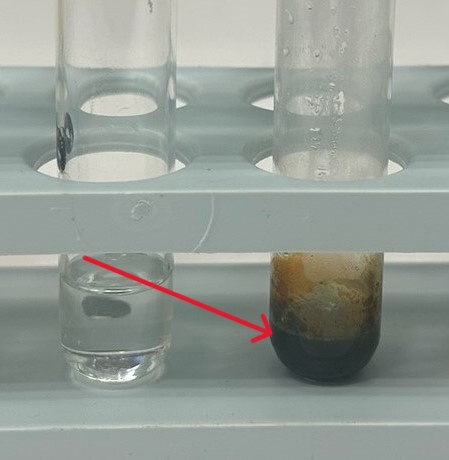
\includegraphics[width=0.75\textwidth]{./media/images/nd_precipitation_reaction_cropped}
    \caption{Neodymium detection reaction. Neodymium is contained in the right sample. The blue precipitate is clearly visible.}
    \label{fig:nd_precipitation}
\end{figure}

\newpage


\subsection{Arsenazo III Assay}

\subsubsection{Arsenazo III}
The arsenazo III assay is based on the dye arsenazo III or ASIII~\cite{arsenazo3assay}.
It is often used to detect calcium, uranium and a lot of other metals, including rare earth elements~\cite{arsenazo3usage, arsenazo3othermetals}.

\begin{figure}[H]
    \centering
    \chemfig[bond style={line width = 1pt}, double bond sep = 3pt]{*6((-S(=[3]O)(=[7]O)-HO)-=(*6(-=(-S(=[1]O)(=[5]O)-OH)-(-N(=[2]N-(*6(=-=-=(-As(=[5]O)(-[1]OH)-HO)-))))=(-OH)--))-=(-OH)-(-N(=[2]N-(*6(=(-As(=[7]O)(-[3]HO)-OH)-=-=-))))=)}
    \caption{Structure of 2,7-bis(2-arsenophenylazo)-1,8-dihydroxynaphthalene-3,6-disulfonic acid. Or, in its abbreviated form, arsenazo III.}
    \label{fig:asiii_structure}
\end{figure}

Arsenazo III was first synthesized in 1959~\cite{arsenazo3fortyyears}.
In comparison to arsenazo I and II, it possesses two functional arseno groups (see figure~\ref{fig:asiii_structure}).
The arsenazo III dye has the property to change its color based on the pH and the presence of some elements.
Normally, the dye has a pinkish-crimson color, but when, for example, thorium is present, the color changes to green.
For other elements, other colors have been reported, such as blue for calcium or violet-blue and also green for rare earth elements (see figure~\ref{fig:asiii_colors}).

\begin{figure}[H]
    \centering
    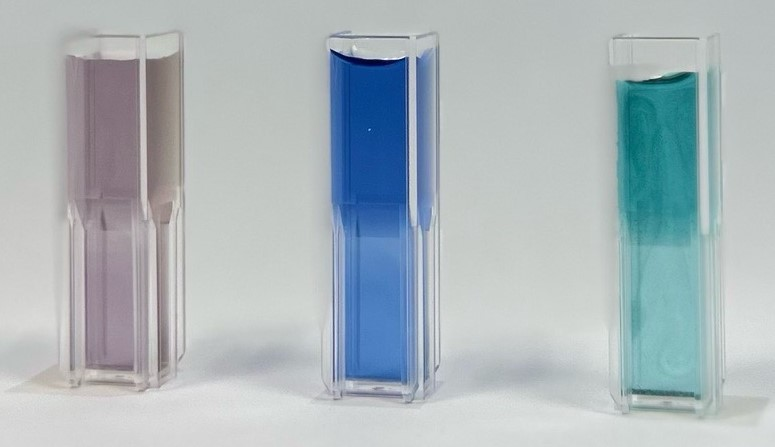
\includegraphics[width=0.9\textwidth]{./media/images/asiii_color_change}
    \caption{Example for different colors of arsenazo III with different samples. The contents of the cuvettes are (from left to right): \ce{FeCl3}, \ce{CuSO4}, \ce{NdCl3}. All are mixed with 10µL of 10mM arsenazo III.}
    \label{fig:asiii_colors}
\end{figure}

The color change happens, because the arsenazo III forms complexes with certain elements.
Arsenazo III and rare earths and some other metals form 1:1 complexes~\cite{arsenazo3complex, arsenazo3structurecomplex}.
This means that for every molecule of arsenazo III, one rare earth element atom was bound (see figure~\ref{fig:asiii_complex_structure}).
The other arseno group is most likely not used to form these stable complexes.


\begin{figure}[H]
    \centering
    \schemestart
    \chemfig[atom sep = 4em, bond style={line width = 1pt}, double bond sep = 3pt]{[:120]*6(-[,,,,dash pattern = on 10pt off 10pt]=(-O?[a])-(-[3]N(=[2]N@{a1}-(*6(=(-As(=[2]O)(-[7,0.7]OH)-O(-[:300,1.5,1,3,dash pattern = on 2pt off 2pt]@{a2}REE?[a,1,{dash pattern = on 2pt off 2pt}]))-[,,,,dash pattern = on 10pt off 10pt]=[,,,,draw=none]-[,,,,draw=none]=[,,,,draw=none]-[,,,,dash pattern = on 10pt off 10pt]))))=[,,,,dash pattern = on 10pt off 10pt])}
    \schemestop
    \chemmove[shorten <=4pt,shorten >=4pt]{
    \draw(a1)..controls +(45:8mm) and +(215:8mm)..(a2);
    \draw[ultra thick] (-1,5.55) rectangle (-1.9,6.05);
    }
    \caption{An arsenazo III complex with an atom of a rare earth element.}
    \label{fig:asiii_complex_structure}
\end{figure}


\subsubsection{Probe Preparation}
To get reliable and correct results, the sample must be prepared beforehand.
This happens by adjusting the pH level of the sample solution to around 2.7 to 2.8.
This ensures that only rare earth ions interact with the arsenazo III dye.
Another advantage of this acidic level is that the ions of the rare earths dissolve better from the sample.

\subsubsection{Measuring REE Concentration}
The measuring of the concentration of the rare earths works with a UV-Vis-spectrometer.
This is a device, that can produce light with a single wavelength.
The light goes through the sample and the light intensity is measured.
When the intensity of the outgoing light \(I\) is set in relation to the intensity of the ingoing light \(I_0\), the emerging result is the transmittance \(T\)~\cite{transmittanceformula}.
\[T=\frac{I}{I_0}\]
The transmittance is then used to calculate the absorbance \(A\) using the following formula~\cite{arbsorbanceformula}.
\[A=\log{T^{-1}}=\log{\frac{I_0}{I}}\]
The absorbance is the output of the UV-Vis-spectrometer.
It is possible to measure just the absorbance at one single wavelength with the device.
However, it can also measure the absorbance from a series of wavelengths and plot the result to a spectrum.
For the Arsenazo III assay, the absorbance at the wavelength of around 650 nm is important (see fig.~\ref{fig:example_spectrum}).
\begin{figure}[H]
    \centering
    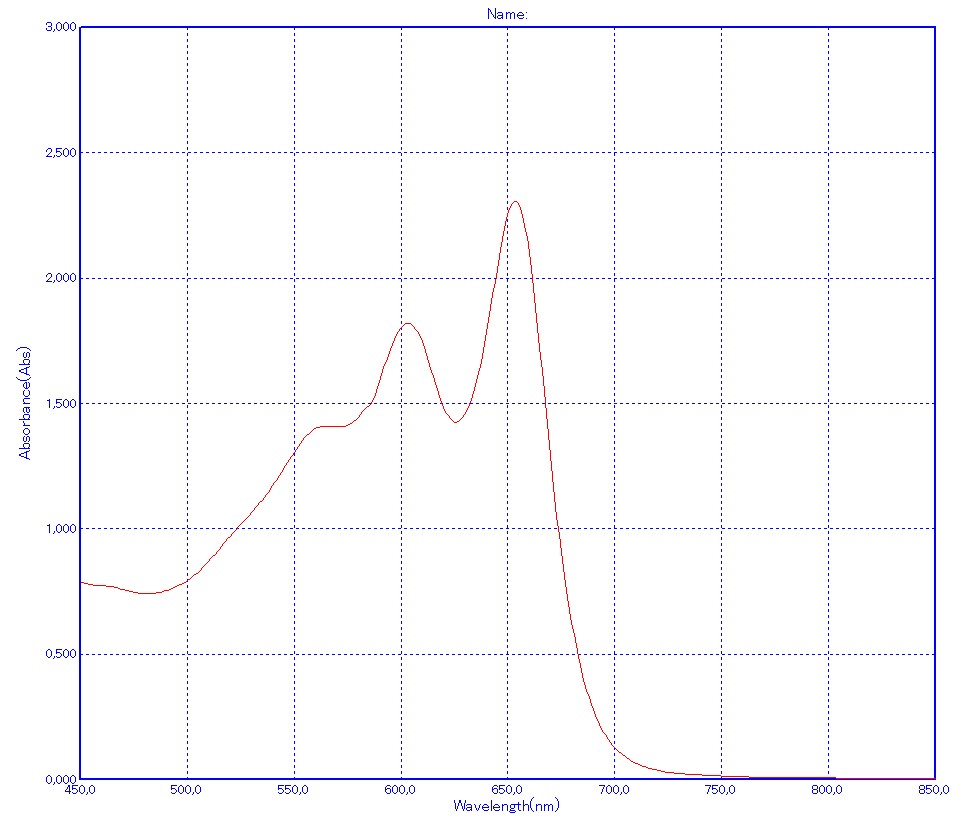
\includegraphics[width=0.9\textwidth]{./media/images/example_spectrum}
    \caption{Example of a spectrum of an arsenazo III assay. The peak at around 650nm is the product of a complex formed by one rare earth atom and one arseno group.}
    \label{fig:example_spectrum}
\end{figure}

The final measurement is done with a 1 mL cuvette.
Half of it is filled with a phosphate-citrate buffer to ensure a correct pH level.
Afterwards, 490 µL of the sample and 10 µL of the Arsenazo III dye are added to the cuvette.
The solutions in the cuvette have to be mixed, and then a spectrum from 500 nm to 800 nm is recorded.
The absorbance at 650 nm is noted.
This is later used for calculation of the concentration.
Then, 20 µL of Arsenazo III are again added and mixed into the cuvette.
The spectrum and the value at the wavelength of 650 nm are again recorded.
The dual measurement is necessary for rare earth concentrations of more than 2µmol/L, because it was found that these values suit better for higher concentrations.

These measurements are not only done with the samples but also with solutions that contain a known concentration of rare earths.
The values can then be used to calculate a calibration line which in turn gives us the concentration of the samples.
    \section{Methylorubrum extorquens}


\subsection{Taxonomy\authorB{}}

\subsubsection{Phylum Pseudomonia}
\emph{Pseudomonadota} is a major phylum of gram-negative bacteria (information about gram-negative bacteria will follow further down).
They are incredibly diverse, encompassing
pathogens, free-living species, nitrogen-fixing bacteria, and many more.
\emph{Pseudomonadota} exhibit a large range of shapes and sizes as well as metabolisms and
habitats which will also be discussed further down.
The diversity of \emph{Pseudomonadota} makes them play a major role in the world's nutrient cycling ranging from crucial ecological relationships with humans to simple things such as nitrogen fixation~\cite{pseudomonadota}.
\emph{Pseudomonadota} includes five classes but only the class \emph{Alphaproteobacteria} is of importance for us.

\subsubsection{Class Alphaprotoebacteria}
\emph{Alphaproteobacteria} is a highly diverse class of bacteria belonging to the phylum \emph{Pseudomonadota}.
They are named after the first letter of the Greek alphabet (alpha) due to being one of the first major lineages to diverge within the \emph{Proteobacteria} phylum.

This class is incredibly varied, encompassing bacteria with a range of lifestyles including phototrophs (light-using), methanotrophs (methane-utilizing), symbionts (mutually beneficial relationships with other organisms), and pathogens (disease-causing).

Soil, water including cold deep-sea vents, hot springs, and symbiotic relationships even
with humans are natural habitats of \emph{Proteobacteria}~\cite{gammaproteobacteria}.

\textbf{Rhizobium:} These bacteria form a symbiotic partnership with legumes, such as peas and soybeans.
\emph{Rhizobium} colonizes the legume's root nodules and fixes atmospheric nitrogen into a usable form that is essential for plant growth.

\textbf{Wolbachia:} This widespread genus of bacteria lives symbiotically within insects and other arthropods.
\emph{Wolbachia} can manipulate the host's reproduction in various ways, sometimes even influencing sex ratios or protecting the host from viruses.

\textbf{Rickettsia:} This genus includes several species that are obligate intracellular pathogens, meaning they can only live and reproduce inside the cells of a host organism.
\emph{Rickettsiae} causes various human diseases, including typhus fever and Rocky Mountain spotted fever.

\textbf{Magnetococcus:} These magnetotactic bacteria contain magnetosomes, specialized
organelles that allow them to align and move along magnetic fields.

\subsubsection{Order Hyphomicrobiales}
\emph{Hyphomicrobiales} can utilize single-carbon compounds like methanol as an energy
source, the bacterium \emph{Methylorubrum} \emph{extorquens} does this, for example.

\emph{Hyphomicrobiales} produce carotenoid pigments and therefore appear pink or orange in colonies.
These colonies are aerobic, which means they require oxygen for growth.
They inhabit a large variety of environments including soils, plant surfaces, root structures, water and dust.

They also play important ecological roles in their habitats, like plant-microbe interactions when metabolizing methanol on plant leaves or carbon and nitrogen cycling in various environments~\cite{methylobacteria_groups}.

\subsubsection{Genus Methylorubrum}
They use specialized pathways to break down methanol for energy and to create biomass.
This metabolic capability has potential applications in Bioremediation, which
means that this bacteria can clean up methanol-contaminated areas.
This family of bacteria is also able to produce valuable chemicals from methanol~\cite{new_methylorubrum}.

Bacteria of the genus \emph{Methylorubrum} are rod-shaped or slightly bent and show pink or
orange pigmentation like every genus that belongs to the order \emph{Methylobacterium.}

\begin{figure}[H]
    \centering
    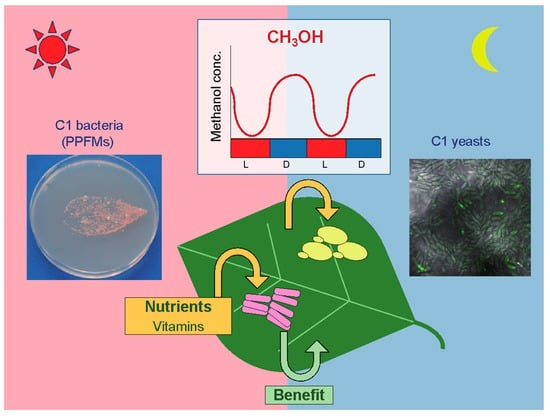
\includegraphics[width=0.9\textwidth]{./media/images/mextorquens_on_leaf}
    \caption{Pink \emph{Methylorubrum extorquens} on a leaf utilizing the plant's nutritiens.}
    \label{fig:mextorquens_on_leaf}
\end{figure}

\subsubsection{Species Extorquens}
In our thesis, the \emph{extorquens} bacterium species holds immense significance as it displays all the key characteristics of the aforementioned groups to which it belongs.
The \emph{Methylorubrum extorquens} strain is unique in its ability to utilize methanol or methane as its sole source of carbon and energy.
Additionally, this bacterium has the capability to metabolize various compounds such as acetate, pyruvate, and succinate, which are converted to energy.
This makes the \emph{Methylorubrum extorquens} strain a particularly fascinating subject for further research and analysis.

\begin{figure}[H]
    \centering
    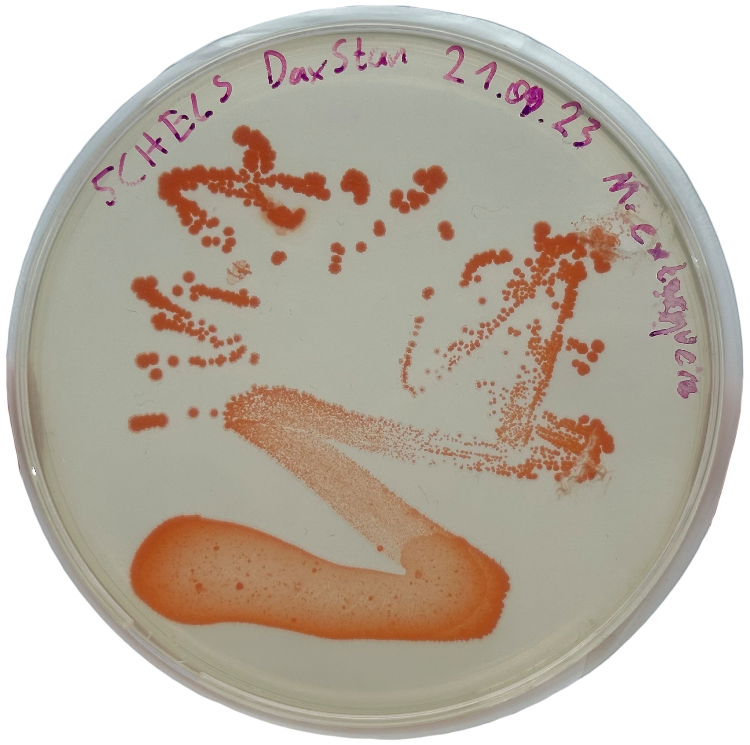
\includegraphics[width=0.8\textwidth]{./media/images/mextorquens_sealed}
    \caption{\emph{M. extorquens} in a sealed petri dish.}
    \label{fig:mextorquens_petri_sealed}
\end{figure}


\subsection{Methanol Metabolism\authorB}
\emph{Methylorubrum extorquens} exhibits the ability to utilize the simple alcohol methanol \ce{CH3OH} as its only source of carbon and energy.
This metabolism is explained in three steps:

\begin{enumerate}
    \item \textbf{Initiation: Oxidation of Methanol}
    \begin{itemize}
        \item Location: Periplasm (the space between the inner and outer cell membranes)
        \item Enzymes:
        \begin{itemize}
            \item Methanol dehydrogenase (MposX):
            \begin{itemize}
                \item XoxF1: Requires lanthanides for activity, oxidizing methanol to
                formaldehyde (\ce{HCHO}) and releasing \ce{H+}.
                \item XoxF2: Less dependent on lanthanides, potentially involved in
                regulating methanol uptake.
            \end{itemize}
        \end{itemize}
        \item Importance: Formaldehyde is a toxic intermediate, requiring rapid conversion for M. extorquens' survival~\cite{methanol_metabolism}.
    \end{itemize}
    \begin{figure}[H]
        \centering
        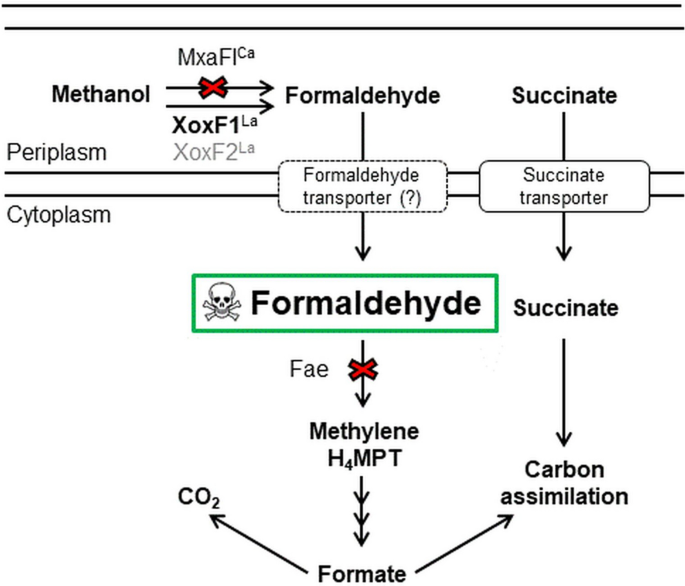
\includegraphics[width=0.9\textwidth]{./media/images/mextorquens_metabolism_methanol}
        \caption{Schematic of the metabolic processes to oxidizing methanol to formaldehyde which is reduced or eliminated and used for growth by cells.}
        \label{fig:mextorquens_metabolism_methanol}
    \end{figure}
    \item \textbf{Capturing the Essence: Fixation of Formaldehyde}
    \begin{itemize}
        \item Molecule: Dephosphotetrahydromethanopterin (\ce{dH4MPT}) acts as a one-carbon
        carrier.
        \item Enzyme: Formaldehyde-activating enzyme (Fae) catalyzes the reaction, attaching
        formaldehyde to \ce{dH4MPT}\@.
        \item Significance: Enables the transport of formaldehyde into the cytoplasm for
        further metabolism~\cite{methanol_metabolism}.
    \end{itemize}
    \item \textbf{Carbon Assimilation: The Serine Cycle Takes Over}
    \begin{itemize}
        \item Location: Cytoplasm
        \item Pathway:
        \begin{enumerate}
            \item Formate dehydrogenase:
            Oxidizes the formaldehyde-\ce{dH4MPT} complex, generating formate (\ce{HCOO}).
            \item Formate acetyltransferase:
            Condenses formate with acetyl-CoA, forming S-acetyl-CoA\@.
            \item Serine hydroxymethyltransferase: Transfers the one-carbon unit from Sacetyl-CoA to glycine, forming serine.
            \item Serine transaminase: Converts serine to pyruvate, a key metabolic
            intermediate.
        \end{enumerate}
        \item Importance: The serine cycle efficiently converts the one-carbon unit from
        methanol into usable cellular building blocks~\cite{methanol_metabolism}.
    \end{itemize}
    \begin{figure}[H]
        \centering
        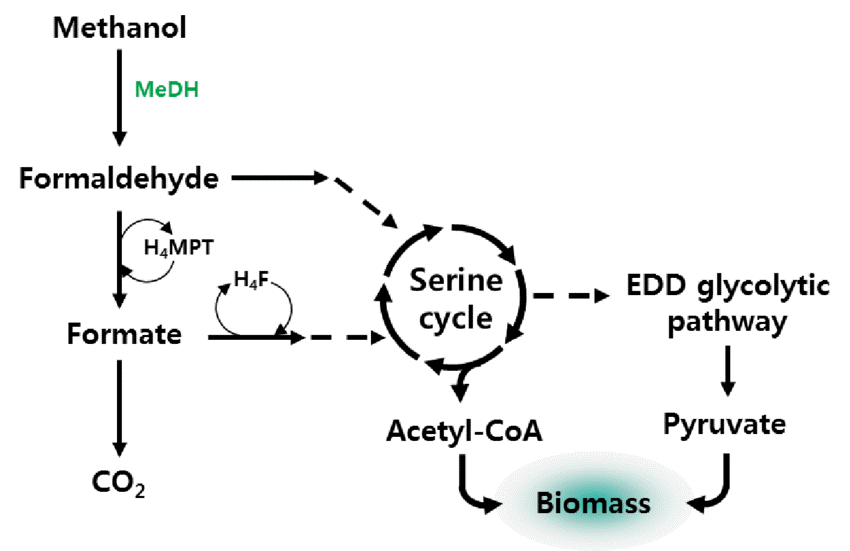
\includegraphics[width=0.9\textwidth]{./media/images/mextorquens_metabolizing_methanol}
        \caption{\emph{Methylorubrum extorquens} metabolizing methanol}
        \label{fig:mextorquens_metabolizing_methanol}
    \end{figure}
\end{enumerate}


\section{Lanmodulin\authorA}
Lanmodulin (LanM) is a protein that was discovered in 2018 in the bacteria \emph{Methylorubrum extorquens}~\cite{lanmdiscovery}.
The molecule is around 12kDa in size, and it possesses unique properties, even when compared to other similar proteins.
Lanmodulin contains four of the so-called EF-hands.
These hands are normally used to sense \ce{Ca^{II}} ions.
Lanmodulin, however, is able to bind \ce{Ln^{III}} and other lanthanide ions (which most of the rare earth elements belong to) to this EF-Hands, not only \ce{Ca^{II}}~\cite{lanmstructure}.

\begin{figure}[H]
    \centering
    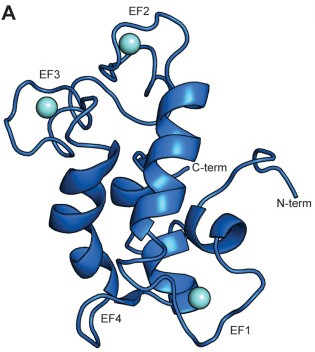
\includegraphics[width=0.6\textwidth]{./media/images/lanm_structure}
    \caption{Graphical visualization of Lanmodulins structure. EF indicates the EF-hands, this is where the REEs can bind to the protein. In this visualization, the turquoise-colored spheres are \ce{Y^{III}} ions which are bound to the EF-hands. Picture from "The biochemistry of lanthanide acquisition, trafficking and utilization", Emily R. Featherston and Joseph A. Cotruvo \cite{lanmroleinbiology}.}
    \label{fig:lanm_structure2}
\end{figure}

The second interesting property originates from the ability to bind lanthanide ions.
It was found that LanM does not only bind lanthanide ions, but it even favors them to bind to its EF-hands.
The affinity for the lanthanides is around \(10^{8}\) times higher than for \ce{Ca^{II}}.
This means that, in a solution with, for example, \ce{Ln^{III}} and \ce{Ca^{II}} ions, only very few calcium ions will bind to the LanM.

When LanM binds the lantanide ions, something interesting happens: it undergoes a transformation.
It changes its shape and morphs into a sphere-like structure, which contains the ions inside.
However, how and why exactly lanmodulin does this, is the subject of ongoing research~\cite{lanmongoingresearch}.

\subsection{Growth\authorB}
\emph{Methylorubrum extorquens} thrives at temperatures between 30°C and 35°C, making it a
mesophilic bacteria.
To promote its optimal growth, the bacteria was placed in a swivel
incubator set to this temperature.
Additionally, the nutrient solution needs to be slightly acidic to neutral, with a pH range of 6.5-7.5, to further enhance growth.
Because \emph{M. extorquens} is an aerobic bacteria, the solution in which it is cultivated must be able to exchange gas and absorb oxygen.
This is achieved by sealing the Erlenmeyer flask with a piece of sterile cotton that allows oxygen to pass through while keeping other bacteria and fungi out.

\begin{figure}[H]
    \centering
    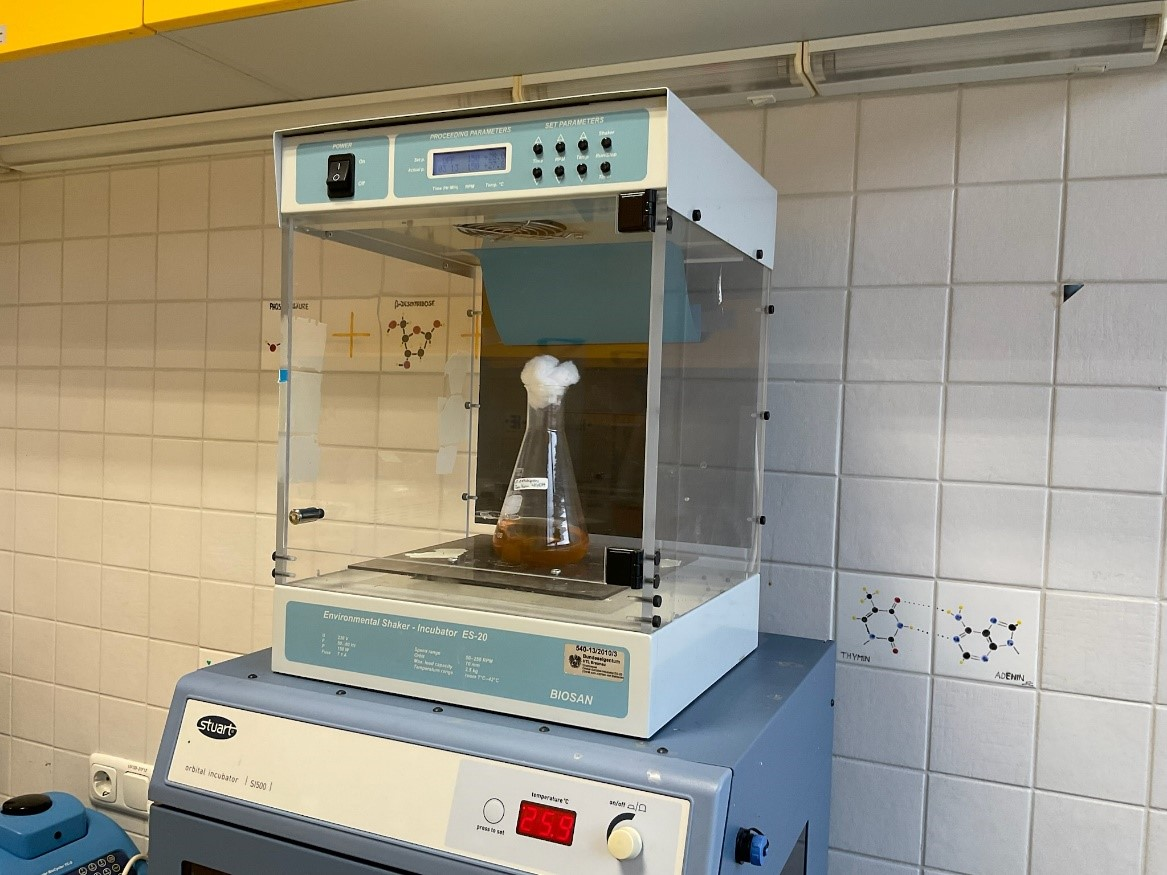
\includegraphics[width=0.9\textwidth]{./media/images/swivel_incubator}
    \caption{Swivel incubator with temperature control used for cultivating \emph{M. extorquens}.}
    \label{fig:swivel_incubator}
\end{figure}

Under optimal conditions, the exponential growth phase of \emph{M. extorquens} typically lasts six to eight hours, during which the number of cells increases rapidly.
However, this growth phase comes to a halt due to a lack of nutrients or waste product accumulation, resulting in the stationary phase.
After this point, the viability and number of cells gradually decrease, known as the death phase.


\subsection{Lysis\authorB}\label{sec:me_lysis}
In order to obtain Lanmodulin and REEs, it is necessary to break open the cell walls of
the bacteria.
This process, known as lysis, can be accomplished using a variety of
techniques - either mechanical or enzymatic.
Mechanical methods include bead beating, French press lysis, and shock freezing, while enzymatic lysis can be achieved through lysozyme treatment, which utilizes an enzyme that specifically breaks down bacterial cell walls.
For this project, a combination of shock freezing and cell wall disruption using an ultrasonic bath was selected.
    \chapter{Protein Extraction/IR-Spectrometry\authorB{}}

    %\chapter{IR-Spectrometry\authorB{}}


    %\chapter{Case Study}

    \chapter{Results and Discussion}

\section{Cultivation of Bacteria\authorB}
Upon acquisition of the bacterial strain, it underwent cultivation on agar plates followed by
incubation. However, initial observations within the first week of incubation did not yield
satisfactory results, as Methylorubrum Extorquens (M. Extorquens) failed to produce a visibly
discernible orange culture indicative of successful growth.
By the third week of cultivation, a distinct orange dot appeared on the surface of the incubated
agar plate, signifying the emergence of bacterial growth. The bacteria were meticulously scraped
from the solid nutrient media for subsequent cultivation in liquid nutrient media, thereby
facilitating a transition from solid to liquid growth conditions.
Subsequent growth in liquid media exhibited a remarkable proliferation of bacterial colonies. To
maintain optimal growth conditions and prevent overpopulation-induced stress, a routine
procedure of decanting 75\% of the liquid culture from the flasks and replenishing them with fresh
liquid media was implemented on a weekly basis. This critical step ensured the sustained viability
and productivity of the bacterial population.
Toward the latter stages of the project, flasks were emptied completely, yet bacterial colonies
regenerated solely from residual deposits adhering to the inner walls of the flasks.
It was also observed that the addition of Methanol had a significant impact on M. Extorquens’
growth speeding up it’s growth by 20\%-50\%, this is explainable by M. Extorquens’ Methanol
metabolizing capabilities.

\section{Protein Analysis\authorA}

\section{Arsenazo-III Assay\authorA}


    \chapter{Project Management}


\section{Planning}\label{sec:planning}

\begin{tabularx}{\textwidth}{ l l l }
    \hline
    \textbf{\textnumero} & \textbf{Milestone}                     & \textbf{Date of Achieval} \\ \hline
    MS\_1                & Cultivation of Bacteria                & 09.11.2023                \\
    MS\_2                & Extraction of LanM                     & 07.12.2023                \\
    MS\_3                & Detection of LanM                      & obsolete                  \\
    MS\_4                & Binding of LanM to Rare Earth Elements & 29.02.2024                \\
    MS\_5                & Separation of Rare Earths from LanM    & n/d                       \\
    \hline
    \caption{Table of planned milestones and their date of achieval.}
\end{tabularx}


\section{Evaluation\authorA{}}

\begin{figure}[H]
    \centering
    \includegraphics[width=0.8\textwidth]{./media/images/teamfoto}
    \caption{The project team}
    \label{fig:teamphoto}
\end{figure}

When we started to conduct some research for the project in the summer break, we also simultaneously began to plan the work with agile project management methods.
As it turned out, doing the project management this way was really helpful.
During our work, we encountered a lot of obstacles which we had not thought of before, which resulted in a slower progress than we had previously expected.

Another problem that we encountered was that we simply could not do our project the way we had planned at the beginning.
Due to limited financial resources and equipment, we could not carry out our planned work.
A lot of methods we tried out did not produce the expected or reliable results.
When we ran into these problems, we had to change how we want to achieve our planned goals.
This also meant that one of our planned milestones (MS\_3 Detection of LanM, see section~\ref{sec:planning}) is completely obsolete, because this step is simply not necessary anymore.

After we had tried our new approach, we finally achieved promising results.
This brought fresh air into the project because we saw that progress was being made.
After weeks of repeated failure, we found new motivation to keep going.

Our new approach requires less expensive resources and is simpler to carry out.
Overall, this made our project better, and it did not change our main goal.
The transformation from our first approach to the other would not have been possible if we had not used agile project management methods.



\newpage


\section{Timesheet}

\subsection{Tobias Daxecker}

\begin{longtable}{|c|p{9cm}|c|}
        \hline
        \textbf{Date} & \textbf{Work} & \textbf{Time in hours}  \\ \endhead \hline
        03.08.2023 & Research & 3,00 \\ \hline
        18.08.2023 & Research & 2,00 \\ \hline
        24.08.2023 & Research & 2,00 \\ \hline
        03.09.2023 & Research & 1,00 \\ \hline
        06.09.2023 & Research & 2,00 \\ \hline
        07.09.2023 & Research & 4,00 \\ \hline
        08.09.2023 & Production of nutrition media & 6,00 \\ \hline
        22.09.2023 & Set up of MS Teams team & 1,00 \\ \hline
        28.09.2023 & Fact sheet, milestones & 1,00 \\ \hline
        02.10.2023 & Research & 1,00 \\ \hline
        06.10.2023 & Freezing of bacteria & 1,00 \\ \hline
        09.10.2023 & Research & 1,00 \\ \hline
        10.10.2023 & Research plan draft, research & 2,00 \\ \hline
        15.10.2023 & Research plan draft, research & 3,00 \\ \hline
        16.10.2023 & Research plan draft, research & 1,00 \\ \hline
        18.10.2023 & Research plan draft, research & 2,00 \\ \hline
        24.10.2023 & Research plan draft, research & 1,00 \\ \hline
        27.10.2023 & Research plan draft, research, newspaper article & 3,00 \\ \hline
        30.10.2023 & Newspaper article, writing of diploma thesis, research & 3,00 \\ \hline
        31.10.2023 & Writing of diploma thesis, research & 4,00 \\ \hline
        01.11.2023 & Writing of diploma thesis, research & 6,00 \\ \hline
        02.11.2023 & Writing of diploma thesis, research & 5,00 \\ \hline
        03.11.2023 & Writing of diploma thesis, research & 5,00 \\ \hline
        06.11.2023 & Writing of diploma thesis, research & 2,00 \\ \hline
        10.11.2023 & Destaining of SDS-PAGE & 2,00 \\ \hline
        12.11.2023 & Newspaper article, writing of diploma thesis & 2,00 \\ \hline
        14.11.2023 & Newspaper article, writing of diploma thesis & 2,00 \\ \hline
        19.11.2023 & Writing of diploma thesis, research & 6,00 \\ \hline
        20.11.2023 & Cultivation of bacteria, writing of diploma thesis, registration for Jugend Innovativ & 3,00 \\ \hline
        24.11.2023 & Destaining of SDS-PAGE, preparation for open house day & 1,00 \\ \hline
        26.11.2023 & Writing of diploma thesis, research & 4,00 \\ \hline
        27.11.2023 & Submission for ECO Bonus & 1,00 \\ \hline
        03.12.2023 & Writing of diploma thesis, research & 3,00 \\ \hline
        10.12.2023 & Writing of diploma thesis, research & 5,00 \\ \hline
        11.12.2023 & Writing of diploma thesis, research & 1,00 \\ \hline
        28.12.2023 & Writing of diploma thesis, research, project report Jugend Innovativ & 3,00 \\ \hline
        29.12.2023 & Writing of diploma thesis, research, project report Jugend Innovativ & 2,00 \\ \hline
        01.01.2024 & Writing of diploma thesis, research & 3,00 \\ \hline
        02.01.2024 & Writing of diploma thesis, research & 4,00 \\ \hline
        03.01.2024 & Writing of diploma thesis, research & 4,00 \\ \hline
        04.01.2024 & Writing of diploma thesis, research & 3,00 \\ \hline
        12.01.2024 & Writing of diploma thesis, research, project report Jugend Innovativ & 1,00 \\ \hline
        14.01.2024 & Writing of diploma thesis, research, project report Jugend Innovativ & 3,00 \\ \hline
        15.01.2024 & Writing of diploma thesis, research, project report Jugend Innovativ & 1,00 \\ \hline
        16.01.2024 & Writing project report for Jugend Innovativ & 3,00 \\ \hline
        17.01.2024 & Writing project report for Jugend Innovativ & 2,00 \\ \hline
        22.01.2024 & Writing project report for Jugend Innovativ & 1,00 \\ \hline
        23.01.2024 & Writing project report for Jugend Innovativ & 2,00 \\ \hline
        24.01.2024 & Writing project report for Jugend Innovativ, review of the project report & 1,00 \\ \hline
        26.01.2024 & Writing project report for Jugend Innovativ & 2,00 \\ \hline
        27.01.2024 & Writing project report for Jugend Innovativ & 6,00 \\ \hline
        27.01.2024 & Writing of diploma thesis & 1,00 \\ \hline
        28.01.2024 & Writing project report for Jugend Innovativ & 1,00 \\ \hline
        30.01.2024 & Writing project report for Jugend Innovativ & 1,00 \\ \hline
        16.02.2024 & Execution of an arsenazo-III assay & 5,00 \\ \hline
        20.02.2024 & Writing of diploma thesis & 2,00 \\ \hline
        21.02.2024 & Writing of diploma thesis & 5,00 \\ \hline
        22.02.2024 & Writing of diploma thesis & 3,00 \\ \hline
        23.02.2024 & Writing of diploma thesis & 3,00 \\ \hline
        26.02.2024 & Writing of diploma thesis & 1,00 \\ \hline
        28.02.2024 & Writing of diploma thesis & 1,00 \\ \hline
        03.03.2024 & Writing of diploma thesis & 4,00 \\ \hline
        04.03.2024 & Writing of diploma thesis & 5,00 \\ \hline
        05.03.2024 & Writing of diploma thesis & 1,00 \\ \hline
        06.03.2024 & Creation of a cost plan & 1,00 \\ \hline
        08.03.2024 & Presentation for job exchange & 1,00 \\ \hline
        10.03.2024 & Presentation for job exchange, Writing of diploma thesis & 2,00 \\ \hline
        11.03.2024 & Presentation for job exchange, Writing of diploma thesis & 1,00 \\ \hline
        17.03.2024 & Writing of diploma thesis & 7,00 \\ \hline

\end{longtable}

\textbf{Total sum of free time work hours: 178,00}

\begin{tabularx}{\textwidth}{l p{1cm} l p{1cm} X}

    Braunau/Inn, \todayshort & & Tobias Daxecker & & \hrulefill                       \\
    \emph{Ort, Datum}        & &                 & & \emph{Unterschrift} \vspace{2cm} \\

\end{tabularx}

\newpage

\subsection{Mathias Standhartinger}

\begin{longtable}{|c|p{9cm}|c|}
    \hline
    \textbf{Date} & \textbf{Work} & \textbf{Time in hours}  \\ \endhead \hline
    03.08.2023 & Research & 3,00 \\ \hline
    18.08.2023 & Research & 2,00 \\ \hline
    24.08.2023 & Research & 2,00 \\ \hline
    03.09.2023 & Research & 1,00 \\ \hline
    06.09.2023 & Research & 2,00 \\ \hline
    07.09.2023 & Research & 4,00 \\ \hline
    08.09.2023 & Production of nutrition media & 6,00 \\ \hline
    06.10.2023 & Freezing of bacteria & 1,00 \\ \hline
    18.10.2023 & Research plan draft, Research & 2,00 \\ \hline
    03.11.2023 & Design of project poster & 2,00 \\ \hline
    03.11.2023 & Registration for contests & 2,00 \\ \hline
    10.11.2023 & Destaining of SDS-Page & 2,00 \\ \hline
    13.11.2023 & Planning of a video for Jugend Innovativ & 2,00 \\ \hline
    14.11.2023 & Newspaper article, writing of diploma thesis & 2,00 \\ \hline
    20.11.2023 & Cultivation of bacteria, writing of diploma thesis & 2,00 \\ \hline
    24.11.2023 & Destaining of SDS-PAGE, preparation for open house day & 1,00 \\ \hline
    29.12.2023 & Writing of diploma thesis, research & 2,00 \\ \hline
    15.01.2024 & Writing of a script for the project video & 2,00 \\ \hline
    16.01.2024 & Writing project report for Jugend Innovativ & 1,00 \\ \hline
    23.01.2024 & Writing of diploma thesis, preparation for video shoot & 4,00 \\ \hline
    24.01.2024 & Writing project report for Jugend Innovativ & 2,00 \\ \hline
    24.01.2024 & Preparation for video shoot & 1,00 \\ \hline
    25.01.2024 & Follow up of video shoot & 1,00 \\ \hline
    27.01.2024 & Design project report for Jugend Innovativ & 4,00 \\ \hline
    28.01.2024 & Design project report for Jugend Innovativ & 2,00 \\ \hline
    29.01.2024 & Correction of the project report & 1,00 \\ \hline
    05.02.2024 & Preparation of video shoot & 2,00 \\ \hline
    07.02.2024 & Writing of a script for the project video and preparation for video shoot & 4,00 \\ \hline
    16.02.2024 & Execution of an arsenazo-III assay & 5,00 \\ \hline
    19.02.2024 & Search for Stockfootage and preparation of video cut & 2,00 \\ \hline
    23.02.2024 & Writing of diploma thesis & 2,00 \\ \hline
    21.02.2024 & Writing of diploma thesis & 4,00 \\ \hline
    26.02.2024 & Writing of diploma thesis & 1,00 \\ \hline
    28.02.2024 & Writing of diploma thesis & 1,00 \\ \hline
    01.03.2024 & Writing of diploma thesis & 3,00 \\ \hline
    02.03.2024 & Writing of diploma thesis & 4,00 \\ \hline
    04.03.2024 & Writing of diploma thesis & 3,00 \\ \hline
    05.03.2024 & Writing of diploma thesis & 3,00 \\ \hline
    06.03.2024 & Creation of a cost plan & 1,00 \\ \hline
    06.03.2024 & Writing of diploma thesis & 4,00 \\ \hline
    07.03.2024 & Writing of diploma thesis & 3,00 \\ \hline
    07.03.2024 & Cutting of the project video & 4,00 \\ \hline
    08.03.2024 & Presentation for job exchange & 1,00 \\ \hline
    08.03.2024 & Cutting of the project video & 4,00 \\ \hline
    11.03.2024 & Presentation for job exchange, Cutting of the project video & 3,00 \\ \hline
    13.03.2024 & Writing of diploma thesis & 3,00 \\ \hline
    14.03.2024 & Writing of diploma thesis & 2,00 \\ \hline
    15.03.2024 & Writing of diploma thesis & 2,00 \\ \hline
    16.03.2024 & Writing of diploma thesis & 3,00 \\ \hline

\end{longtable}

\textbf{Total sum of free time work hours: 120,00}

\begin{tabularx}{\textwidth}{l p{1cm} l p{1cm} X}

    Braunau/Inn, \todayshort & & Mathias Standhartinger & & \hrulefill                       \\
    \emph{Ort, Datum}        & &                        & & \emph{Unterschrift} \vspace{2cm} \\

\end{tabularx}


    \chapter{Future Work\authorB{}}

To further optimize this endeavor for industrial applicability, several imperative steps must be
undertaken. Primarily, there is a critical need to augment the efficiency of bacterial proliferation and
the resultant yield of Rare Earth Elements (REEs). Achieving this entails the development of
innovative methodologies aimed at curtailing the growth duration and nutrient utilization by
Methylorubrum Extorquens. Moreover, the primary substrate for bacterial metabolism, methanol,
could be replaced with its more rudimentary and economically advantageous precursor, methane,
which is also amenable to metabolization by M. Extorquens. To realize the full-scale industrialization
of this project, rigorous testing in expansive bioreactor systems is indispensable, alongside the
incorporation of diverse forms of Electronic Waste.
Determining the most economically viable category of E-Waste necessitates extensive experimental
evaluation. Concurrently, alongside the E-Waste assessments, there arises a pressing need for the
development of a high-capacity, efficient, and durable shredding apparatus tailored to handle various
types of E-Waste. This undertaking poses multifaceted challenges, particularly in terms of safety and
cost considerations. An industrial-grade E-Waste shredder must be inherently non-combustible and
proficient in processing metal, plastic, fiberglass, and adhesive materials, all while maintaining
optimal power consumption levels and facilitating facile maintenance protocols.
    \chapter{Related Work\authorA{}}

There are some other studies that are somewhat close to our work.
Most of them have the same basic idea at their core.
That is to use \emph{M. extorquens} or lanmodulin to recycle rare earth elements.

\begin{figure}[H]
    \centering
    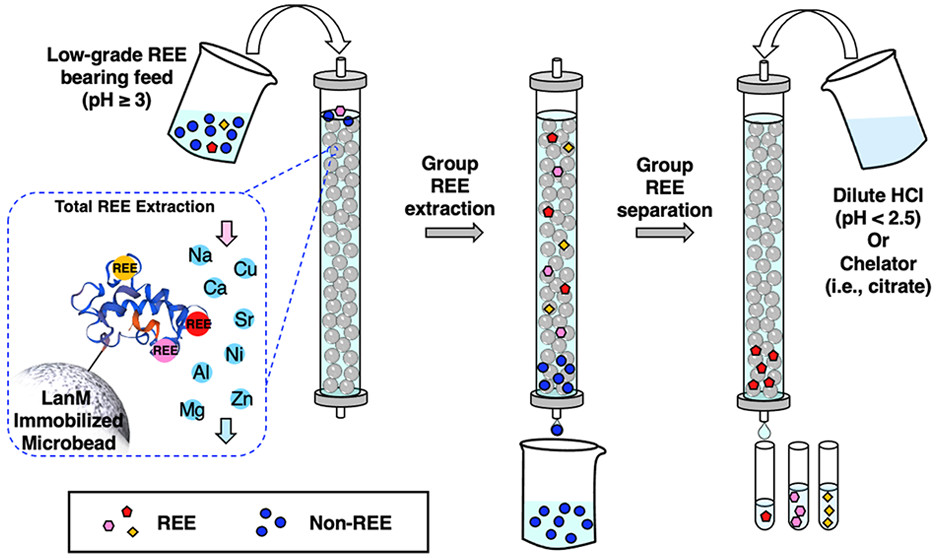
\includegraphics[width=0.8\textwidth]{./media/images/original_study_process}
    \caption{Overview of the work which inspired this thesis.
    Picture from "Bridging Hydrometallurgy and Biochemistry:
    A Protein-Based Process for Recovery and Separation of Rare Earth Elements", Dong et al.~\cite{originalstudy}.}
    \label{fig:original_study_process}
\end{figure}

An example for the usage of only lanmodulin would be the work of Dong et al.~\cite{originalstudy}.
Their approach was to take lanmodulin and attach it to a microbead (a small sphere made of agarose).
The product of this procedure is the immobilized lanmodulin.
They made a lot of the immobilized lanmodulin and put it into a column.
Afterwards, they let a solution which contained ash from a coal power plant, which in turn contained some REEs, flow through the column.
The REEs get caught by lanmodulin, and every other metal flows freely through the whole column.
After that, they washed their column, and then they began separating the different rare earths.
They achieved this by giving solutions with different pH values into their column.
Lanmodulin releases only some certain rare earths at a certain pH which is useful for separating them.
When every rare earth has been extracted, the column can be cleaned and even be reused for the next recycling process.

This is a very clever process that even inspired this thesis.
However, this work is not easy to reproduce.
It requires costly chemicals and machinery, which only a company or a university can afford.
Therefore, it was not feasible at our school.
What must also be taken into consideration is that they used a genetically modified bacteria which produced the lanmodulin.
This alone would fill a whole diploma thesis.

\newpage

Good et al. took another approach, which is surprisingly similar to our work.
Their basic idea was to let \emph{M. extorquens} grow in a solution which contains electronic waste and find methods to increase the yield of this recycling method~\cite{similarwork}.
This approach is fairly similar to our own work.
However, this work did not inspire us because the paper was first published on December 27th 2023, when we already had worked three months on our project.

\begin{figure}[H]
    \centering
    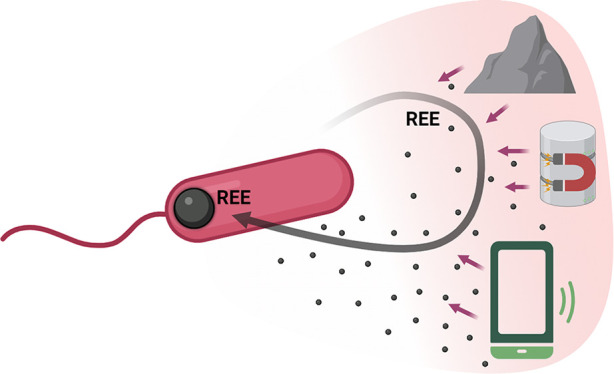
\includegraphics[width=0.8\textwidth]{./media/images/similar_work}
    \caption{Very simplified abstract of the work from Good et al.
    Picture from "Scalable and Consolidated Microbial Platform for Rare Earth Element Leaching and Recovery from Waste Sources", Good et al.~\cite{similarwork}.}
    \label{fig:similar_work}
\end{figure}

The main difference to our work is their technological advantage.
They used a genetically modified strain of \emph{M. extorquens} AM1, which is called \(\Delta\)\emph{mxaF}.
They deleted the gene \emph{mxaF} to ensure that the growth of the bacteria is dependent on the uptake of rare earths.
This led to a higher rare earth uptake capacity per bacteria.

Another remarkable difference is that they did not only let the bacteria grow with crushed magnets, but also with a crushed smartphone.
This did have, interestingly, no significant impact on the growth of \emph{M. extorquens} AM1 \(\Delta\)\emph{mxaF}, according to their study.

After that, they improved the yield by adding an organic acid to the bacteria's growth medium.
This helped to extract the rare earths from the crushed magnet (and smartphone).
What also boosted their yield was that they genetically engineered \emph{M. extorquens} AM1 \(\Delta\)\emph{mxaF} even further.

    \chapter{Conclusion}



    \appendix

    \chapter*{Acknowledgements}
\addcontentsline{toc}{chapter}{Acknowledgements}

\textbf{<Taste L>}

    %\addcontentsline{toc}{chapter}{Listings}
    %\lstlistoflistings

    \addcontentsline{toc}{chapter}{List of Figures}
    \listoffigures


    \addcontentsline{toc}{chapter}{Bibliography}
    \bibliographystyle{unsrt}
    \bibliography{literature}

    
\chapter*{CV} \markboth{CV}{CV}
\addcontentsline{toc}{chapter}{CV}


\htlParagraph{Tobias Daxecker}

\renewcommand{\arraystretch}{1.2}
\begin{tabularx}{1\textwidth}{@{} l X l @{}}

\emph{Geburtstag, Geburtsort:} & 25.11.2004, Braunau am Inn & 
\multirow{5}{2.5cm}{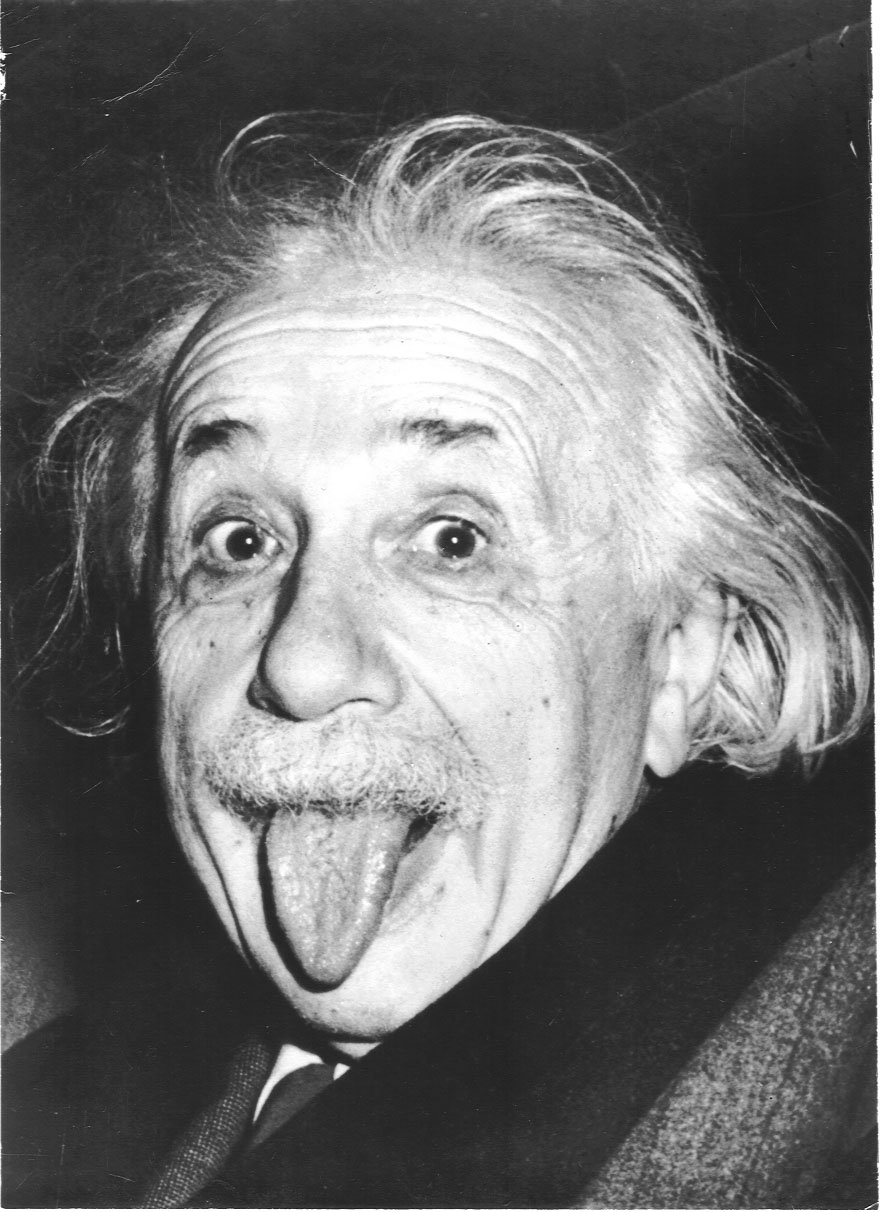
\includegraphics[width=2.5cm]{./media/images/einstein.jpg}
} 
\\
\emph{Schulbildung:} & Volksschule \newline Neue Mittelschule \newline HTL & \\
\emph{Praktika:} & Firmenname, Zeit, Tätigkeit & \\
\emph{Anschrift:} & Adenberg 19\newline 5144, Handenberg\newline Österreich & \\
\emph{E-Mail:} & tobias.daxecker@htl-braunau.at & \\

\end{tabularx}
\\\\


\htlParagraph{Mathias Standhartinger}

\begin{tabularx}{1\textwidth}{@{} l X l @{}}
\emph{Geburtstag, Geburtsort:} & 28.12.2004, Braunau am Inn & 
\multirow{5}{2.5cm}{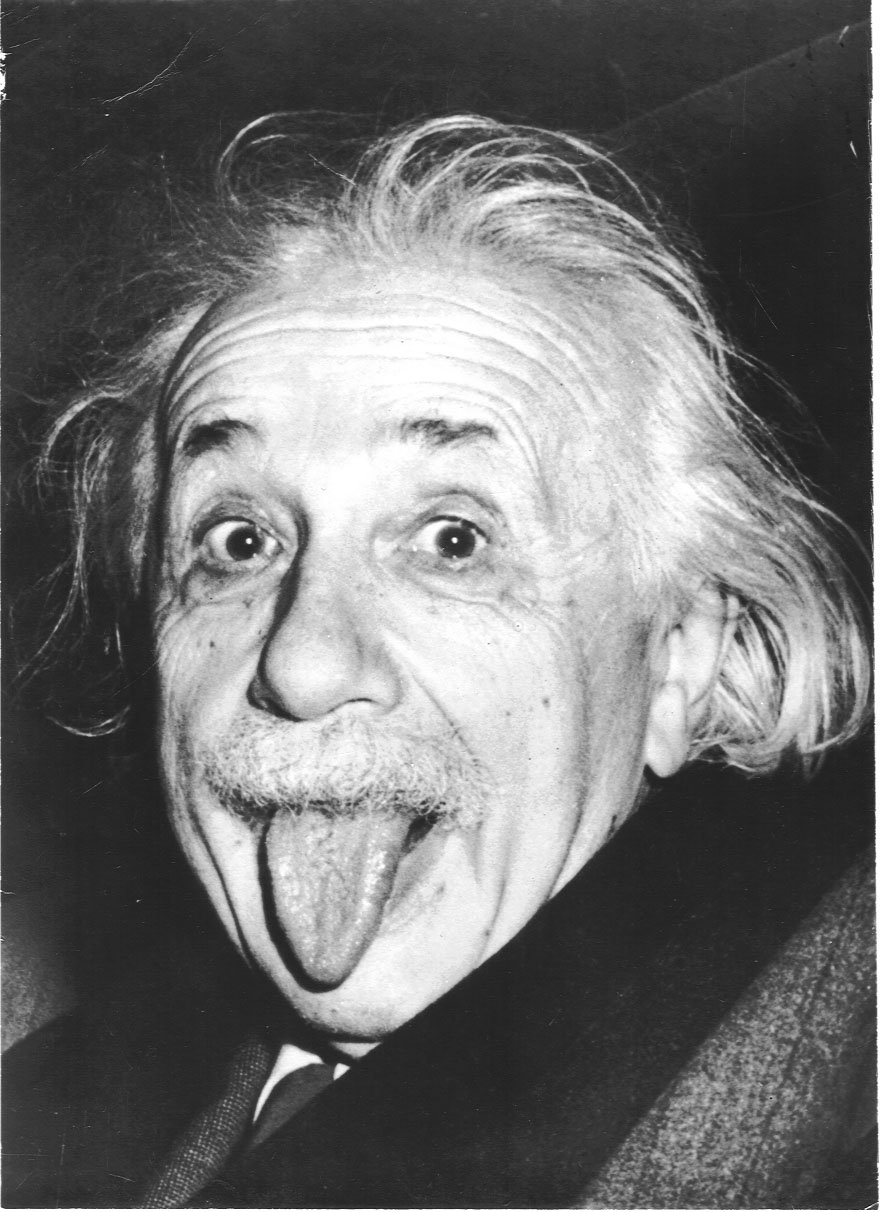
\includegraphics[width=2.5cm]{./media/images/einstein.jpg}
} 
\\
\emph{Schulbildung:} & Volksschule \newline Neue Mittelschule \newline HTL & \\
\emph{Praktika:} & Firmenname, Zeit, Tätigkeit & \\
\emph{Anschrift:} & Strasse Nummer\newline PLZ, Ort\newline Österreich & \\
\emph{E-Mail:} & max@mustermann.com & \\

\end{tabularx}



\end{document}